%!TEX root = thesis.tex


\chapter{Introduction and Background}
\label{chapter1}

\section{Introduction}

Controllers allow systems to perform desired functions and reduce the need for human intervention to achieve the desired behavior.
%
As technology advances,
complex processes are being automated more often, which increases
the need for more complex and sophisticated control systems.
%
However, designing control systems to provide full autonomy for complex problems is often difficult using conventional control design methods. For this reason, control systems may be designed for a subsystem in order to provide partial autonomy.
%
For instance, modern automobiles can have multiple levels of autonomy from cruise control to lane-stay assist to self-driving, each requiring control of multiple subsystems to provide the desired level of autonomy.
%
Domain knowledge of the system used in the control application is necessary in order to design appropriate controllers.
%
This domain knowledge includes how to model the system, how to choose and design appropriate performance metrics, as well as knowledge of how different controllers affect the behavior of the system.
% \rnotes{Somehow make this stronger?}
%

Controllers are generally designed to optimize specific performance metrics. For the cruise control example, this may include minimizing fuel usage or minimizing settling time of the velocity of the vehicle with constraints on passenger comfort. For some simple systems, the optimal control problem can be solved analytically.
%
For instance, Linear Quadratic Regulator (LQR) control is a common method for solving the optimal control problem for linear systems with quadratic cost functions. Methods such as this can also be used for nonlinear systems if they are linearized~\cite{Dogan:2005a,Khan:2020a}.
%
For general nonlinear systems, especially those with discontinuous nonlinearities
% \rnotes{only those with discontinuous nonlinearities?}
and those operating in dynamic, unstructured environments that are difficult to model, there are no general methods for analytically solving the optimal control problem. For these types of systems, optimal controllers are often approximated through recursive or iterative methods. One of these methods is reinforcement learning (RL).

Reinforcement learning is a class of methods in which control policies are learned through repeated interaction with the system\cite{Sutton:2018a,Li:2017a}. This allows RL to learn online without needing domain knowledge of the laws that govern the system. This is useful for applications that are not amenable to analytical solutions for optimal controllers.
% This may even be done directly on a physical system or when there is no dynamic model of the system since RL only requires samples of the state of the system for each action. \rnotes{Give some examples for which RL would be a useful control method.}
However, there are drawbacks that prevent widespread application of RL beyond simulation and laboratory settings.
RL is sample inefficient, requiring many interactions with the system, meaning that significant training time is often required to learn a usable policy. RL policies are also black boxes, and it is often difficult to interpret the control laws governing their behavior.
% with \rph{large numbers of parameters} representing the control laws.
%
This is especially true for high degree-of-freedom systems or those with continuous-action spaces where it is necessary to utilize neural networks to learn the control policy.
% \rnotes{Elaborate about neural networks being like a black box?}
Additionally, it is usually impossible to generate performance guarantees for control policies generated using RL.
RL policies for which there are no performance guarantees or that are not interpretable will not be utilized in safety-critical applications such as transportation or health care~\cite{Cheng:2019a,Hart:2019a,Tambon:2022a}.
%
For these reasons, the use of RL is primarily reserved for simulation and laboratory settings where the risks from poorly performing policies can be minimized.
%
% \rph{Controllers that combine RL elements with conventional control elements can provide controllers with the ability to be }
%
% Since conventional control methods do not require training and their performance can be more easily verified, 
Since conventional control methods do not have the same drawbacks as RL,
%
it is beneficial to combine conventional control methods with RL to generate controllers that reduce the drawbacks of conventional control and RL when used separately.

There have been methods proposed to utilize RL agents along with conventional closed-form control methods~\cite{Wang:2007a,Johannink:2019a,Silver:2018a}. However, there is no work that provides comprehensive design guidelines.
The primary goal of this dissertation is to provide guidelines for designing controllers that combine RL and conventional control methods utilizing domain knowledge.
% This work will provide guidelines for designing combined controllers that:
% This work provides guidelines for using domain knowledge to:
These guidelines facilitate using domain knowledge of control theory to:
% With this work, these methods will allow for combined controllers to be designed that:
\begin{itemize}
	\item design RL controllers that reduce required training time to achieve desirable performance compared to training RL without domain knowledge
	\item design RL controllers that provide an initial policy that is safe to use on a physical system before training the agent
	\item train policies that provide bounds on stability and can be analyzed using  conventional stability analysis tools
	\item interpret policy behavior according to conventional control analysis methods
\end{itemize}
%
The above contributions will allow RL to be more readily applied for physical systems since shorter training time and good initial policies make training directly on physical systems more feasible.
%
Additionally, generating policies that can be interpreted and that have performance and stability guarantees makes RL more attractive for safety-critical applications.
% \rph{Learning policies that can be analyzed for stability and being able to interpret the behavior of the policy will make RL more attractive for safety-critical systems where no one would use the control policy without understanding how the system would respond in different situations.}

The remainder of this chapter introduces the background for analytical solutions for optimal control, as well as describing the limits of analytical solutions that motivate the use of approximate optimal control and RL methods.
% \rph{The rest of this chapter includes a background for analytical optimal control, approximate optimal control, and RL.}
Section~\ref{sec:optimal_control_overview} describes conventional optimal control methods for dynamic systems, including analytical and approximation methods. Section~\ref{sec:RL_overview} provides an overview of RL and describes the noteworthy developments leading to modern RL algorithms. Deep RL is then described in Section~\ref{sec:deep_RL_overview}, followed by drawbacks of using RL in Section~\ref{sec:RL_drawbacks}.  An overview of the combined controller methods proposed in this work is presented in Section~\ref{sec:combined_control_overview}.

\section{Optimal Control}
\label{sec:optimal_control_overview}
The optimal control problem requires finding a control law that optimizes a performance metric subject to the system dynamics and other constraints. It is widely used in many applications ranging from robotics to economics~\cite{Lewis:2012a}.
%
% Depending on the application and the simplifications that can be made to a system model to make the optimal control problem possible to solve analytically,
Formulations for the optimal control problem can be categorized based on their applicability to discrete-time and continuous-time systems.

\subsection{The Discrete-Time Problem}
A discrete-time system is one in which the input and output signals do not vary continuously, but instead vary only at non-infinitesimal intervals. Although most systems vary continuously, continuous systems are typically controlled using discrete controllers. Discretizing the system can also simplify analysis. The state evolution of a discrete-time system is described by:
%
\begin{equation}
x_{k+1}=f(x_k,u_k)
\label{eq_chap1:discrete_EOM}
\end{equation}
%
where $x_{k+1}$ and $x_k$ are the next state and current state, respectively, and $u_k$ is the current input at time step $k$. The general form of a cost function defining the performance metric to be minimized is:
%
\begin{equation}
J_i(x_i)=\phi(N,x_N)+\sum_{k=i}^{N-1}L(x_k,u_k)
\label{eq_chap1:discrete_cost}
\end{equation}
%
where $L(x_k,u_k)$ is the intermediate cost at time step $k$ and is dependent on the current state and input. The fixed final cost, $\phi(N,x_N)$, is dependent on the final time step, $N$, and final state, $x_N$. Equation~\eqref{eq_chap1:discrete_cost} defines the cost incurred during the interval $[i,N]$. The goal of solving the optimal control problem is to find a control policy, $u_k^*$, that minimizes \eqref{eq_chap1:discrete_cost} on the time interval $[i,N]$. For discrete-time systems, this can be accomplished by converting the optimal control problem into a static optimization problem and solving for the optimal control sequence, $[u_i^*, u_{i+1}^*, \dots, u_{N-1}^*]$, that minimizes $J$ subject to \eqref{eq_chap1:discrete_EOM}. This method is sometimes employed in approximate solutions methods such as Model Predictive Control (MPC), but the optimization must be performed for every initial condition since it does not result in a closed-form control law.

\subsection{The Continuous-Time Problem}
%
Continuous-time systems describe the continuous state evolution of the output based on a continuous input.
% \rph{Most physics-based applications, such as robotics, are modeled in continuous time.}
The general form describing the state evolution of a continuous-time system is:
%
\begin{equation}
\dot{x}(t) = f(x,u,t)
\label{eq_chap1:cont_EOM}
\end{equation}
%
where $x$ is the current state at time $t$, and $\dot{x}(t)$ is the time derivative of $x(t)$ dependent on the current state, $x$, current input, $u$, and current time, $t$. The general form of the cost function for the continuous-time problem is:
%
\begin{equation}
J(t_0)=\phi(x(T),T) + \int_{t_0}^TL(x(t),u(t),t) \, \text{d}t
\label{eq_chap1:cont_cost}
\end{equation}
%
where $\phi(x(T),T)$ is the fixed final cost at the final time, $T$, and $L(x(t),u(t),t)$ is the intermediate cost. Equation~\eqref{eq_chap1:cont_cost} defines the cost from any initial time, $t_0$, to the final time, $T$. The goal of the continuous-time optimal control problem is to find a continuous control policy, $u^*(t)$, that minimizes the cost on the time interval.
For simple or simplified optimal control problems, the discrete-time and continuous-time optimal control problems can be solved analytically. For instance, the process of solving \eqref{eq_chap1:cont_cost} for linear continuous-time systems with quadratic intermediate cost, $L(x(t),u(t),t)$, results in LQR. In other cases, the solution must be approximated. The following sections describe common solution methods for the optimal control problem.


\subsection{Dynamic Programming}
Dynamic programming was originally developed by Richard Bellman during the 1950s.
It relies on the principle that the optimal policy must have the property that no matter the previous control decisions, the remaining control decisions must be optimal~\cite{Bellman:1957a}.
%In other words, the control policy is optimal from any state that results from previous control actions from the optimal policy.
This allows the optimal control problem to be solved recursively.

% You can solve discrete-time bellman equation analytically, but continuous-time HJB must be approximated.

Using this notion to define the optimal control problem recursively, the cost function for discrete-time systems \eqref{eq_chap1:discrete_cost} can also be defined from any time step, $k$:
%
\begin{equation}
J_k(x_k) = L(x_k,u_k) + \phi(N,x_N)+\sum_{k=i}^{N-1}L(x_{k+1},u_{k+1}) = L(x_k,u_k) + J_{k+1}(x_{k+1})
\label{eq_chap1:discrete_cost_recursive}
\end{equation}
%
where the cost of being in the current state, $J_k(x_k)$, is the intermediate cost in the current state, $L(x_k,u_k)$, plus the sum of all future cost from the next state, $J_{k+1}(x_{k+1})$. If the optimal control sequence from state $x_{k+1}$ is known, $J^*_{k+1}(x_{k+1})$, then the optimal cost in state $x_k$ is:
%
\begin{equation}
J^*_k(x_k)= \min_{u_k}(L(x_k,u_k)+J^*_{k+1}(x_{k+1},u_{k+1}))
\label{eq_chap1:discrete_cost_optimal}
\end{equation}
For systems without constraints, \eqref{eq_chap1:discrete_cost_optimal} is used to analytically solve for the optimal control law.
%
In the case where there are constraints that make analytical solutions of \eqref{eq_chap1:discrete_cost_optimal} impossible, the problem can still be solved numerically.

Dynamic programming can also be used to solve the optimal control problems for continuous-time systems. Following the principle analogous to \eqref{eq_chap1:discrete_cost_recursive}, the cost from any state, $x$, at time, $t$, described by \eqref{eq_chap1:cont_cost}, can be reformulated as:
%
\begin{equation}
J(x,t)=\phi(x(T),T) + \int_{t}^{t+\Delta t}L(x,u,\tau) \, \text{d}\tau + \int_{t+\Delta t}^{T}L(x,u,\tau) \, \text{d}\tau
\label{eq_chap1:cont_cost_recursive1}
\end{equation}
%
where the integral of the intermediate cost from $[t,t+\Delta t]$ is the cost from the current state at time $t$ to a new state after a short time $\Delta t$. The final cost, $\phi(x(T),T)$, and the integral of intermediate cost from $[t+\Delta t, T]$ is the cost, $J(x+\Delta x,t+\Delta t)$, from the next state, $x+\Delta x$, at the next time, $t+\Delta t$, such that \eqref{eq_chap1:cont_cost_recursive1} can be written as:
%
\begin{equation}
J(x,t)=\int_{t}^{t+\Delta t}L(x,u,\tau) \, \text{d}\tau + J(x+\Delta x, t+\Delta t)
\label{eq_chap1:cont_cost_recursive2}
\end{equation}
%
If the optimal cost, $J^*(x+\Delta x, t+\Delta t)$, is known, then the optimal cost for all $x$ and $t$ is,
%
\begin{equation}
J^*(x,t)=\min_{u(\tau)} \left[ \int_{t}^{t+\Delta t}L(x,u,\tau) \, \text{d}\tau + J^*(x+\Delta x, t+\Delta t) \right]
\label{eq_chap1:cont_cost_optimal}
\end{equation}
%
Although it is possible to use \eqref{eq_chap1:cont_cost_optimal} to numerically solve for optimal policies, it cannot be solved analytically.
% \rph{there is no straightforward way to analytically solve it.}
Instead, it is common to manipulate \eqref{eq_chap1:cont_cost_optimal} such that it is more amenable to analytical solutions:
%
\begin{equation}
-\frac{\partial J^*}{\partial t} = \min_{u(t)}\left(L + \left(\frac{\partial J^*}{\partial x}\right)^T f \right)
\label{eq_chap1:HJB}
\end{equation}
%
This is known as the Hamilton-Jacobi-Bellman (HJB) equation. It is a partial differential equation for the optimal cost, and its solution provides the optimal control policy for any system. For LTI systems with quadratic cost functions, the HJB equation can be used to derive the Linear Quadratic Regulator (LQR).
% ~\pc[original LQR paper and applications].
However, it is usually impossible to solve \eqref{eq_chap1:HJB} analytically for nonlinear systems with constraints and non-quadratic cost functions. This has motivated the creation of methods to numerically solve for the solution to the HJB equation~\cite{Beard:1997a,Beard:1998a,Boulbrachene:2001a,SaberiNik:2012a}.
% \rnotes{We could also use viscosity solutions~\cite{Bardi:1997a}.} \rnotes{Why is that? Find an explanation and/or sources.}

Even for the cases in which the solution of the HJB equation can be approximated, it must be solved offline because it is recursive.
% This prevents solving for optimal controllers in real-time.
% while the system is being implemented.
% The following section introduces methods that have been developed to directly approximate solutions for optimal controllers that can be solved online and forward-in-time.
The following section introduces online and forward-in-time methods to directly approximate solutions for optimal control problems.

% \rnotes{Even though this may eventually give us a good approximate solution, it must still be solved recursively (I would guess). These recursive methods still cannot be used online. They must be solved offline and then applied to the system.}

% \rnotes{Explain why it is difficult (impossible?) to find analytical solutions for HJB. Explain why I may not want to use HJB directly. For instance, it is recursive. Since I generally can't get analytical solutions, I may want to use other methods for online solutions, i.e. ones that can be solved forward in time. Also discuss any other problems with it. Then go right on with explaining the other approximation methods.}

\subsection{Forward-in-Time Solutions}
% There are a few methods that are useful if you want to approximate solutions to the optimal control problem online or forward in time.

One commonly used online optimal control method is Model Predictive Control (MPC), which approximates solutions for the optimal control problem by directly solving for a control sequence that optimizes a cost function over a finite horizon~\cite{Schwenzer:2021a}. It is able to approximate solutions for the general optimal control problem for nonlinear systems and for systems with constraints. To determine an optimal control sequence, a model of the system dynamics is necessary in order to predict the state evolution of the system with respect to the optimal input sequence. At each time step, the first input in this sequence is passed to the system, then the process is repeated at the next time from the next state. While, in theory, MPC can be implemented for any system, its use is limited by its computational complexity. Since MPC does not solve for a closed-form control law, the control sequence must always be solved online.
%
Although online solutions are often not challenging for systems with low bandwidth, it is a challenge for high-bandwidth systems since the time to compute the optimal sequence over the finite horizon can cause significant delay.
% The computational complexity \rph{may not be a problem} for systems with low bandwidth, but it would be a problem for systems with higher bandwidth 

Another approximation method is Iterative LQR (iLQR), which is an extension of LQR for optimal control of nonlinear systems.
% Iterative LQR (iLQR) is another approximation method for nonlinear optimal control problem~\pc. \rph{It is an extension of LQR, which finds optimal controllers for LTI systems utilizing quadratic cost functions. 
% \rnotes{It may also be a direct descendant of Differential Dynamic Programming?}
iLQR adapts standard LQR for the general optimal control problem by linearizing the system at the current state. The cost function also needs to be approximated as a quadratic, often by using Taylor approximation taken to two terms. The optimal gains for the current linearization and approximated cost function are then solved using the formulation as in standard LQR. For the next state at the next time step, the linearization of the system and quadratic approximation of the cost function are repeated.
%
This method works well for unconstrained nonlinear systems with general cost functions. Unlike MPC, however, since iLQR is based on LQR, it cannot be solved for systems with hard constraints on state and control inputs. However, there are modifications to iLQR proposed to solve constrained problems~\cite{ChenJ:2019a}.

MPC provides a way to handle constraints while optimizing. However, it is necessary to perform computationally expensive numerical optimization at every time step to generate an optimal control sequence over a finite horizon. iLQR simplifies the control problem into one in which the optimal control input at the current time can be found analytically, which reduces computational complexity compared to MPC.
However, the standard implementation does not account for systems with constraints.
This motivates the development of optimal control methods to handle general constraints with low computational complexity during implementation. Reinforcement learning is one method that solves these problems.

\section{Reinforcement Learning}
\label{sec:RL_overview}
\subsection{Reinforcement Learning Overview}

% \begin{itemize}
% 	\item RL basics
% 	\begin{itemize}
% 		\item Basic RL diagram
% 		\item Markov Decision Process
% 		\begin{itemize}
% 			\item States
% 			\item Actions
% 			\item Reward
% 		\end{itemize}
% 	\end{itemize}
% 	\item Tabular RL
% 	\begin{itemize}
% 		\item RL used to have to be done tabularly
% 		\item This required discretizing state and action spaces
% 		\item \textit{Figure: RL table}
% 		\item Q-learning
% 		\item \textit{Figure: graphical example of how Q-learning works}
% 	\end{itemize}
% 	\item Deep RL
% 	\begin{itemize}
% 		\item Value-based methods
% 		\begin{itemize}
% 			\item RL uses Neural networks to approximate the value function
% 			\item This allows learning with continuous observation spaces
% 		\end{itemize}
% 		\item Policy-based methods
% 		\begin{itemize}
% 			\item Does this allow the use of continuous action spaces?
% 		\end{itemize}
% 		\item Actor-Critic methods
% 		\item DDPG
% 		\item TD3
% 	\end{itemize}
% \end{itemize}

%
\begin{figure}[tb]
\begin{center}
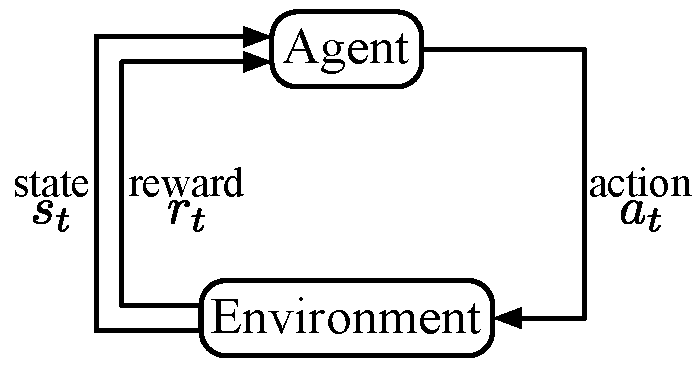
\includegraphics[width = 0.5\textwidth]{figures/figures_introduction/RL_diagram.pdf}
\caption{Basic reinforcement learning process} 
\label{fig_chap1:RL_diagram}
\end{center}
\end{figure}
%

% \rnotes{Transition from the previous section. How does RL solve the problems indicated in the previous section? RL can be implemented model-free. Once trained, RL is not computationally complex/does not require constant online optimization. }

Reinforcement learning (RL) is an iterative forward-in-time method to solve for optimal control policies.
% \rnotes{RL is loosely based on biological/animal learning.}
RL combines concepts from psychological studies on trial-and-error learning with optimal control theory. Algorithms for RL are able to generate optimal policies through repeated trial-and-error interaction with an environment.
% \rph{RL relies on Markov Decision Process. This has states and rewards.}
This is illustrated graphically in the diagram of the basic learning process for RL shown in Figure~\ref{fig_chap1:RL_diagram}. The learning process has two main components which exchange information. The agent is analogous to a controller in conventional controls terminology, and the environment is analogous to the plant. The agent generates an action, $a_t$, or control input, in accordance with the current policy. This action is passed to the environment. The state, $s_t$, of the environment changes as a result of the action.
%
During training, a reward signal is used to quantify the value of the current action in the current state; this is similar to a cost function in conventional optimal control. When the reward signal is passed to the agent, the policy is updated in order to progressively maximize the reward.
%
% A reward signal is used to quantify how good the policy is. The state and reward are passed to the agent so that it can update its policy and try a new action.
This is usually repeated for a set number of repetitions or episodes.
% \rnotes{Say something about this being for training only?}
Once training is complete, the approximated optimal control policy is implemented in closed form without further online optimization.
% Once training is complete, the control input at any time step is found in closed form without need for further optimization as with MPC.
% \rnotes{Somehow mention action space and observation space, probably by mentioning Markov Decision Process.}

% \rnotes{The equations below probably don't belong here. This section should be more qualitative, while the sections about the specific algorithms are more quantitative.}

RL is based on the same principles as dynamic programming.
While an optimal control policy is found in dynamic programming by minimizing a cost function, RL finds optimal policies by maximizing cumulative reward or return from the policy:
%
\begin{equation}
R(s_0) + \gamma^1R(s_1) + \dots +  \gamma^NR(s_N)
\end{equation}
%
where $R(s)$ is the incremental reward received from being in state $s$ and $\gamma$ is a discount rate between $0$ and $1$. This reward is used to evaluate the performance of the policy along a state trajectory $[s_0, s_N]$. It is useful to use cumulative reward to evaluate the policy from any state, $s_n$.
%
This allows the agent to generate policies that are optimal over a longer horizon since a state that produces low incremental reward may later lead to states that produce high reward when following the current policy. However, the cumulative reward that will be received after the current state is usually not known and is instead approximated.
%
The expected cumulative reward or return is defined as the value of being in state, $s_n$, and following the current policy, $\pi$:
% The value of the policy at any state $s_n$ is the expected reward that will be received from that state and future states when following a policy, $\pi$:
%
\begin{equation}
V^\pi(s_n) = \mathbb{E}\left[\sum_{n=0}^N \gamma^n R(s_n) \right]
\label{eq_chap1:expected_return}
\end{equation}
%
where $\gamma$ is the discount rate between $0\leq \gamma \leq 1$ that adjusts the current value of future rewards.
% where $\gamma$ is a discount rate such that the expected return is finite even for infinite episodes \rnotes{I think}.
Because value discounting is exponential due to $\gamma^n$, \eqref{eq_chap1:expected_return} can be written recursively:
%
\begin{equation}
% V^\pi(s_n) = R(s_n) + \mathbb{E}\left[\sum_{n=0}^N \gamma^{n+1} R(s_{n+1}) \right]
V^\pi(s_n) = \mathbb{E}\left[R(s_n) + \sum_{n=0}^N \gamma^{n+1} R(s_{n+1}) \right]
\label{eq_chap1:expected_return_recursive}
\end{equation}
%
This is analogous to the recursive Bellman equation from \eqref{eq_chap1:discrete_cost_recursive} since the current value at state $s_n$ is a function of the expected future value from state $s_{n+1}$.
%
These concepts are also applicable to stochastic systems.
% The derivation for standard value-based RL for stochastic systems is analogous to the derivation of the equations used in dynamic programming.
For stochastic systems, the probability of transitioning from state $s$ to state $s'$ given the action, $a$, is:
%
\begin{equation}
\text{Prob}[s'|s,a]=P_{ss'}[a]
\end{equation}
%
Modifying \eqref{eq_chap1:expected_return_recursive} for use with stochastic systems results in:
%
\begin{equation}
V^{\pi}(s)=R(\pi(s))+\gamma\sum_{s'}P_{ss'}[\pi(s)]V^{\pi}(s')
\label{eq_chap1:Q-learning_value}
\end{equation}
%
where $R(\pi(s))$ is the reward gained by performing an action according to the policy, $\pi$, in state $s$.
%
% Equation~\eqref{eq_chap1:Q-learning_value} is recursive since the value of the current state, $V^{\pi}(s)$, depends on the value of the future state, $V^{\pi}(s')$.
% \rph{Apparently, Bellman and Dreyfus and then some guy named Ross tell us}
The optimal value of the current state corresponding to the optimal policy, $\pi^*$, is:
%
\begin{equation}
V^*(s) = V^{\pi^*}(s) = \max_a \left[ R(\pi^*(s))+\gamma\sum_{s'}P_{ss'}[\pi^*(s)]V^{\pi^*}(s')\right]
\label{eq_chap1:Q-learning_op_value}
\end{equation}
%
Many algorithms that rely on using the value function to approximate future reward have been developed, each with distinct advantages and disadvantages. The following sections discuss algorithms that have been noteworthy contributions to the field of RL.
% \rph{Since RL is a class of methods that rely on \eqref{eq_chap1:expected_return_recursive} to find optimal policies, there are many algorithms that have been designed. Each algorithm has distinct advantages and disadvantages. The following sections explain different popular algorithms.}

% \subsection{Markov Decision Process}

\subsection{Q-Learning}

%
\begin{figure}[tb]
\begin{center}
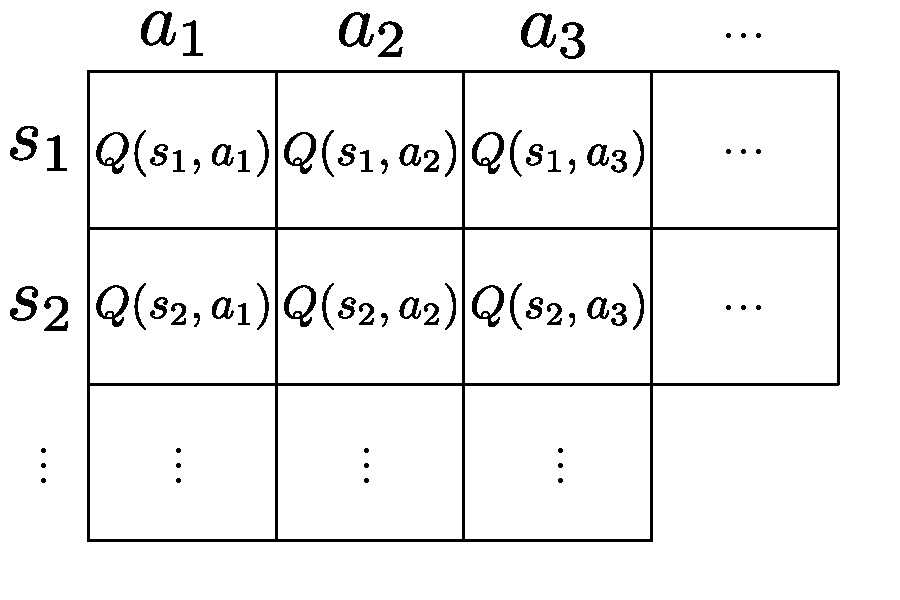
\includegraphics[width = 0.5\textwidth]{figures/figures_introduction/Q_table.pdf}
\caption{Example Q-table} 
\label{fig_chap1:Q_table}
\end{center}
\end{figure}
%

Q-learning is a tabular method for model-free RL~\cite{Watkins:1989a,Watkins:1992a,Clifton:2020a}.
%
The primary advantage of Q-learning compared to previous algorithms is the reduction in computational complexity of updating the policy during training.
%
Since the goal of RL is to iteratively optimize the policy, multiple versions of the policy must be evaluated. The value of being in each state will depend on the policy being used, such that a new policy would require the value function under that policy to be reevaluated for every state. Q-learning modifies how the value of a state is calculated, such that modifying the policy does not require recalculating the value function for every state, thus reducing the computational complexity of evaluating new policies. The action-value function represents the value of applying any action, $a$, at the current state, $s$, then following the policy, $\pi$, thereafter:
%
\begin{equation}
Q^\pi(s,a) = R(a)+\gamma\sum_{s'}P_{ss'}[\pi(s)]V^{\pi}(s')
\end{equation}
%
This is used to aggregate a Q-table that stores the evaluation of the action-value function for all combinations of states and actions, as illustrated in Figure~\ref{fig_chap1:Q_table}.
Q-learning allows the action-value function, $Q$, to approximate the optimal action-value function independently of the current policy.
% This allows the value of the current state and action to be evaluated without invalidating the value of the next state, $V^{\pi}(s')$.
This provides a way to incrementally update the existing Q-table without needing to regenerate a new table for every policy update.
%
% \rnotes{Edit and refine this. Add formula for updating Q-values. Find citations for other implementations/explanations.}
%
The success of Q-learning motivated the development of other algorithms that utilize action-value functions~\cite{Jang:2019a}.
%
However, because Q-learning is a tabular method, it suffers from the ``curse of dimensionality.'' The Q-learning algorithm has to experience every combination of state and action repeatedly. This is problematic for high dimensional problems such as multi-degree-of-freedom systems or multiple-input systems. This also makes it difficult to use for continuous problems since the system must be discretized to be solved by Q-learning. These challenges motivated the introduction of general function approximation methods to represent the value and action-value for any combination of state and action~\cite{Baird:1995a,Xu:2014a}.

\section{Deep Reinforcement Learning}
\label{sec:deep_RL_overview}
% \rnotes{Who was the first to try deep RL?}
Although tabular RL methods often work well for problems with discrete action and observation spaces, tabular methods are restrictive for high-dimensional problems since the size of the tables need to increase with the size of the action and observation spaces, which increase computational complexity to find optimal policies. This restriction also prevents tabular RL from being used for continuous action and observation spaces. 
% Using tabular methods is restrictive for reinforcement learning.
% It usually works just fine for small problems with discrete action spaces and observation spaces, but the tables would have to be very large for problems with more action and observation spaces~\pc.
This issue is solved by using nonlinear function approximators.
% Function approximation can be thought of as an instance of supervised learning~\pc.
Neural networks are commonly employed as nonlinear function approximators for machine learning and have been used extensively in supervised learning and unsupervised learning~\cite{Alloghani:2020a}. RL is referred to as deep RL when a deep neural network is used to approximate the value function or policy. Neural networks in deep RL are able to mitigate the ``curse of dimensionality'' by directly approximating the nonlinear value function.
%
Whereas tabular methods require every combination of observation and action to be visited, using a neural network to approximate the value function generates continuous estimates of the value. This eliminates the need to visit every observation and allows a continuous observation space to be used.
%
One of the first successful deep RL algorithms was used to train agents to play Atari games, where the agents were trained directly from pixel data. These agents trained using deep RL were often able to match or surpass human performance~\cite{Mnih:2015a,Shao:2019a}.
%
These contributions have enabled the development of other RL algorithms to train agents for other high-dimensional problems.

%
\begin{figure}[tb]
	\begin{center}
	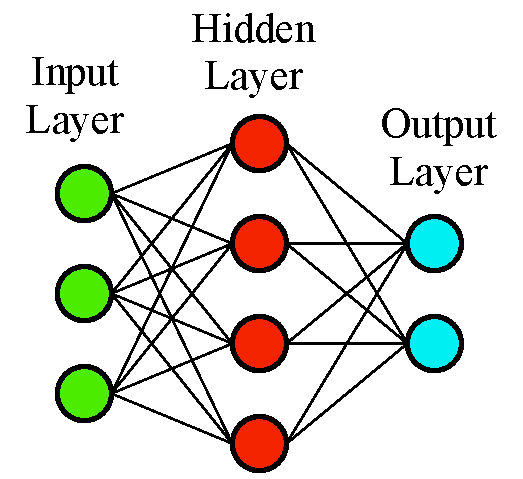
\includegraphics[width = 0.55\textwidth]{figures/figures_introduction/Neural_network_diagram.pdf}
	\caption{Neural network diagram} 
	\label{fig_chap1:NN_diagram}
	\end{center}
\end{figure}
%
An illustration of a neural network is shown in Figure~\ref{fig_chap1:NN_diagram}.
%
Neural networks are comprised of nodes which each have input and output signals.
%
Nodes of a neural network are arranged in layers. Nodes within each layer are not connected to each other, but each node is connected to nodes in the previous and following layer.
%
Each connection between the nodes is associated with a real-valued weight, and the value of the output signal from each node is computed from the value of the input signal and the weight of the connection.
%
The green nodes represent the input layer. In the case of RL, the input layer accepts the observations. The blue nodes represent the output layer. In RL, the outputs of the network can be the value in a state or the actions in the case of an actor-critic algorithm. The red nodes represent the hidden layers.
%
Although the number of nodes in the input and output layers are determined by the application, the number of hidden layers and the number of nodes in each hidden layer of deep neural networks can vary.
%
Networks with fewer nodes in the hidden layers have fewer parameters with which to approximate the value function. Increasing the size of the network generally allows the deep neural network to better approximate the value function due to having more parameters to adjust to get a good fit~\cite{Bengio:2009a}.
% This is what ``deep'' refers to in deep neural networks.
% \rnotes{and the activation function?}


% The sizes of the input and output layers of a neural network are determined by the application. For RL, the size of the input layer must match the number of observations and the size of the output layer must match the number of actions passed to the environment. The number of hidden layers and number of nodes in each hidden layer can vary.
% Deep neural networks with fewer nodes have fewer parameters with which to approximate the value function. Increasing the size of the network generally allows the deep neural network to better approximate the value function due to having more parameters to adjust to get a good fit~\cite{Bengio:2009a}.

% \rnotes{Discuss backpropagation for NN updates?}

There are many deep RL algorithms that have been developed. The main categories include value-based methods and actor critic methods. Noteworthy algorithms from these categories are described in the following sections.

% The return is the sum of the discounted future reward:
% \begin{equation}
% R=\sum_{t=0}^{t=\infty}=\gamma^t r(s_t,a_t
% \label{eq_chap1:reward_func}
% \end{equation}
% %
% where $\gamma$ is the discount factor and $r(s_t,a_t$ is the reward function.

% Value function:
% \begin{equation}
% V^\pi(s)
% \label{eq_chap1:value_func}
% \end{equation}

% Q-value function:
% \begin{equation}
% Q^\pi(s,a)
% \label{eq_chap1:Q-value_func}
% \end{equation}

\subsection{Value-Based Methods}
Value-based deep RL algorithms replace the tabular evaluation of the value or action-value function with a deep neural network capable of approximating continuous functions. This enables learning policies for systems with many observations or continuous observation spaces.
%
One of the first and most influential deep RL algorithms is the Deep Q-network (DQN) algorithm~\cite{Mnih:2013a,Mnih:2015a}.
DQN is based on the standard Q-learning algorithm with modifications that enable the use of deep neural networks to approximate the nonlinear action-value function.
%
% \rph{Linear function approximation methods had been used previously since training with nonlinear function approximators was unreliable.}
% DQN is based on the standard Q-learning algorithm, which is a tabular method, but includes a deep network to approximate the value function.
%
The use of deep neural networks allowed DQN to learn to play Atari games directly from raw pixel input. 
%
DQN produced performance comparable or superior to humans for four of the seven Atari games tested.
%
% \rnotes{DQN was shown to be able to learn to play Atari games directly from raw pixel input from an emulator. DQN produced performance comparable or superior to humans for four of the seven Atari games tested. It is an off-policy algorithm and does not require the network to be trained with data from the current policy. For off-policy algorithms, experience replay is used to store state-action samples from training into a replay buffer. A minibatch is sampled from the replay buffer for each network update phase. This improves data efficiency since past data can be used multiple times during training. This also reduces the correlation between samples used during each network update phase.}
%
Although DQN is able to operate on continuous observation spaces, it requires discrete action spaces since every action must be evaluated to find the optimal action from each state. This motivated the development of methods that can directly model the optimal policy.
% \rnotes{This is because DQN uses $\epsilon$-greedy policy?}

\subsection{Actor-Critic Methods}

%
\begin{figure}[tb]
\begin{center}
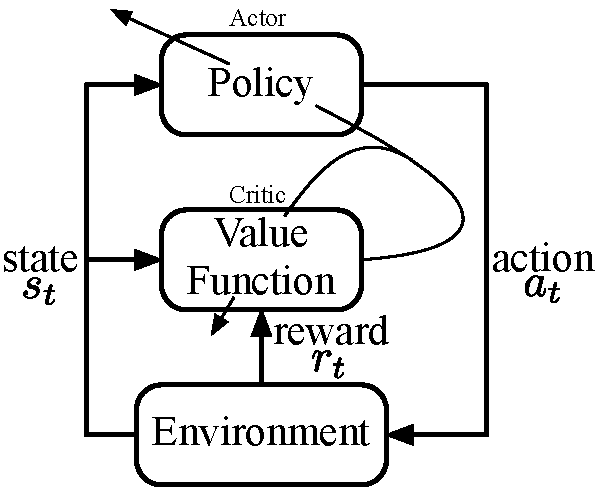
\includegraphics[width = 0.5\textwidth]{figures/figures_introduction/Actor_Critic_diagram.pdf}
\caption{Actor-critic diagram}
\label{fig_chap1:AC_diagram}
\end{center}
\end{figure}
%

% \rnotes{Prioritize explaining the specific equations used for actor critic methods.}
%
% \rph{The use of neural networks to approximate the value function allows continuous observation spaces to be used since every combination of states and actions do not need to be explored to determine its value. However, action spaces are still required to be discrete since every action must be tried to determine the optimal policy over a state-evolution. A function defining the actions to be used is necessary to provide a continuous action space.}
One method to directly learn policies is to model them using deep neural networks.
Using a function approximator such as a neural network to model the policy allows inputs from observations to produce actions in a continuous action space.
%
% Continuous action spaces can be achieved by using a neural network directly to approximate a policy.
One type of RL algorithm that takes advantage of neural networks to produce both continuous action spaces and continuous observation spaces is an actor-critic algorithm, where the value function and policy are modeled using separate neural networks~\cite{Lillicrap:2016a,Fujimoto:2018a}.
% Actor-critic algorithms don't rely on calculating an action based on the neural network parameterizing the value function.
% One network is used to learn the value function, another network is used to learn the policy.
A diagram illustrating the basic function of an actor-critic algorithm is shown in Figure~\ref{fig_chap1:AC_diagram}. The actor portion of the algorithm contains the policy and provides the action to the environment. The critic contains the network that approximates the value function. Both the actor and critic networks must be progressively updated to produce accurate estimates of the expected cumulative reward as well as the optimal policy that maximizes the reward.
% \rnotes{So, what are the limitations of DQN?}

% \rnotes{Generalized policy iteration may be important to know about here~\pc[Sutton and Barto 1998].}

%%%%%%%%%%%%%%%%%%%%%%%%%%%%%%%%%%%%%%%%%%%%%%%%%%%%%%%%%%%%%%%%%%%%%%%%%%%%%%%%%%%%%%%%%%

% \rph{The standard way to generate the policy from the approximation of the value or action-value is not useful for continuous action spaces modeled by neural networks, as in actor-critic. This is often achieved by using greedy maximization. This is fine for discrete, low-dimensional action spaces, but it is problematic for continuous action spaces since greedy maximization requires global maximization. It is more convenient to change the policy based on the gradient of the action-value network. This was first proposed by Sutton et al.~\cite{Sutton:1999a}. \what{This allows for the policy to be moved in the direction of optimal iteratively at each evaluation without having to perform optimization on every parameter at every evaluation?} Policy gradient improves reliability to converge towards locally optimal policies. \what{There was then work done to allow this to be done for deterministic policies~\cite{Silver:2014a}}. Policy updates rely on changing the parameters of the policy based on the gradient of the performance, i.e. the reward.} \rnotes{Get some of the equations from deterministic policy gradient, and explain in one or two sentences why it is advantageous over stochastic policy gradient.}

% The equations that are important for actor-critic algorithms are:

% Policy gradient:
% \begin{equation}
% \nabla_\theta J(\theta)\approx\mathbb{E}_{\tau}\sum_{t=0}^{T-1}\nabla_\theta \log \pi_\theta(a_t|s_t)A_{\pi_\theta}
% \label{eq_chap1:policy_gradient}
% \end{equation}
% %
% where $A_{\pi_\theta}$ is the advantage function. \rnotes{I think maybe for algorithms like DDPG and other Q function based algorithms, $G_t$ is replaced with the Q-value, $Q_t$}. The advantage function is:
% %
% \begin{equation}
% A_{\pi_\theta}(s_t,a_t)=r(s_t,a_t)+V_{\pi_\theta}(s_{t+1})-V_{\pi_\theta}(s_{t})
% \label{eq_chap1:advantage_func}
% \end{equation}
% %
% The policy parameters are updated by:
% %
% \begin{equation}
% \theta=\theta+\alpha\nabla_\pi J(\theta)
% \label{eq_chap1:actor_update}
% \end{equation}
% %
% and the critic parameters are updated by:
% %
% \begin{equation}
% \omega=\omega+\alpha\delta_t
% \label{eq_chap1:critic_update}
% \end{equation}
% %

%%%%%%%%%%%%%%%%%%%%%%%%%%%%%%%%%%%%%%%%%%%%%%%%%%%%%%%%%%%%%%%%%%%%%%%%%%%%%%%%%%%%%%%%%%

\subsection{Deep Deterministic Policy Gradient}
% \rnotes{Check this against DDPG and TD3. Find more detail on policy gradient and the one for value updates.}
% \rnotes{Should I make this less technical?}
A noteworthy development in actor-critic algorithms came from the development of the Deep Deterministic Policy Gradient (DDPG) algorithm~\cite{Lillicrap:2016a}.
% One of the algorithms used for this work is Deep Deterministic Policy Gradient (DDPG).DDPG is an actor-critic method that neural networks for both the actor and critic. This allows DDPG to be used for high-dimensional continuous state and action spaces.
The critic portion of DDPG is inspired by Deep Q Network (DQN)~\cite{Mnih:2013a,Mnih:2015a}. The actor portion of DDPG is updated based on the Deterministic Policy Gradient (DPG), which allows the policy to be updated based on the gradient of the value function~\cite{Silver:2014a}.

%%%%%%%%%%%%%%%%%%%%%%%%%%%%%%%%%%%%%%%%%%%%%%%%%%%%%%%%%%%%%%%%%%%%%%%%%%%%%%%%%%%%%%%%%%

% The policy gradient can be calculated by \rnotes{I think this is actually stochastic}:
% %
% \begin{equation}
% \nabla_{\theta^\mu}J\approx \frac{1}{N}\sum_i\nabla_aQ(s,a|\theta^Q)|_{s=s_i,a=\mu(s_i)}\nabla_{\theta^\mu}\mu(s|\theta^\mu)|s_i
% \end{equation}
% %
% The deterministic policy gradient is:
% %
% \begin{equation}
% \nabla_{\theta}J(\mu_\theta) = \mathbb{E}_{s\sim\rho^{\mu}} [\nabla_\theta\mu_\theta(s) \nabla_a Q^\mu(s,a)|_{a=\mu_\theta(s)}]
% \end{equation}
% %
% The policy parameters are updated by \rnotes{Is this right?}:
% %
% \begin{equation}
% \theta=\theta+\alpha\nabla_\pi J(\theta)
% \label{eq_chap1:actor_update}
% \end{equation}
% %
% The critic is updated by minimizing the loss as in Q-learning:
% %
% \begin{equation}
% L=\frac{1}{N}\sum_i(y_i-Q(s_i,a_i|\theta^Q))^2
% \end{equation}
% %
% where $y_i$ is the target value:
% %
% \begin{equation}
% y_i=r_i+\gamma Q'(s_{i+1},\mu'(s_{i+1}|\theta^{\mu'})|\theta^{Q^'})
% \end{equation}
% %
% \rph{This equation seems to basically be a correction for the Q-function using the current reward instead of the Q-value with the current state and action.
% It is apparently very important to have target networks, $Q'$ and $\mu'$, because you are trying to calculate the target value using, $y_i$, using $Q$, but $Q$ is also being updated. This makes $Q$ prone to divergence if target networks are not used~\cite{Mnih:2013a}.}

%%%%%%%%%%%%%%%%%%%%%%%%%%%%%%%%%%%%%%%%%%%%%%%%%%%%%%%%%%%%%%%%%%%%%%%%%%%%%%%%%%%%%%%%%%

\subsection{Twin-Delay DDPG}
A common disadvantage of deep RL algorithms is the occurrence of overestimation. This occurs when the algorithm overestimates the value approximation, often resulting in suboptimal policies. 
% \rph{Although DDPG provided a way to learn optimal policies for continuous observation and action spaces, this algorithm has a problem with overestimation. This overestimation is common for algorithms using function approximation and often leads to suboptimal policies.}
The Twin-Delay DDPG (TD3) algorithm is a modification of the DDPG algorithm that limits the occurrence of overestimation~\cite{Fujimoto:2018a}. This is accomplished by using two critic networks, where the policy is updated according to the critic with the lowest value estimate to avoid overly optimistic updates.
% Twin-Delay DDPG (TD3) uses a pair of critic networks to limit overestimation.
%
This makes the action-value estimates more accurate to more reliably find optimal policies.
% \rph{One critic network is updated frequently while the other is updated with a delay. This makes the action-value estimates more reliable since it is less susceptible to abrupt changes in the action-value.}

\section{Problems with RL}
\label{sec:RL_drawbacks}
%
Although RL has advantages over other methods for approximating optimal controllers, it also has drawbacks that have prevented its widespread adoption.
%
One of the primary drawbacks is the iteration needed to train policies, which often requires significant training time. This is illustrated by Figure~\ref{fig_chap1:long_training_time} showing reward during training. At the beginning of training, the policy performs poorly and produces low reward. This not only corresponds to a suboptimal policy but may also indicate that the policy causes unsafe behavior or does not perform the desired task, making it unusable. More training time is required before the policy achieves a suitable threshold of performance to allow it to be implemented for its intended purpose.

The tendency to perform poorly in the initial stage of training is a drawback that prevents training directly on physical systems. For instance, using a poorly performing policy on a robotic system may result in the system behaving in a way that causes it to damage itself or its surroundings.
The iteration required during training also reduces the feasibility of training on physical systems since this may require significant human supervision to reset the system for each iteration or if a failure occurs due to the poor performance. Training in simulation is faster and can be more easily automated to require less human supervision.
%
However, agents trained in simulation often have degraded performance when transferred to physical systems due to modeling error and sensor noise.
There has been a large amount of research performed to bridge the gap between simulation and physical applications, or sim-to-real~\cite{Peng2018a,Zhao:2020a}. This often requires initially training in simulation then completing training on the physical system.

%
\begin{figure}[tb]
\begin{center}
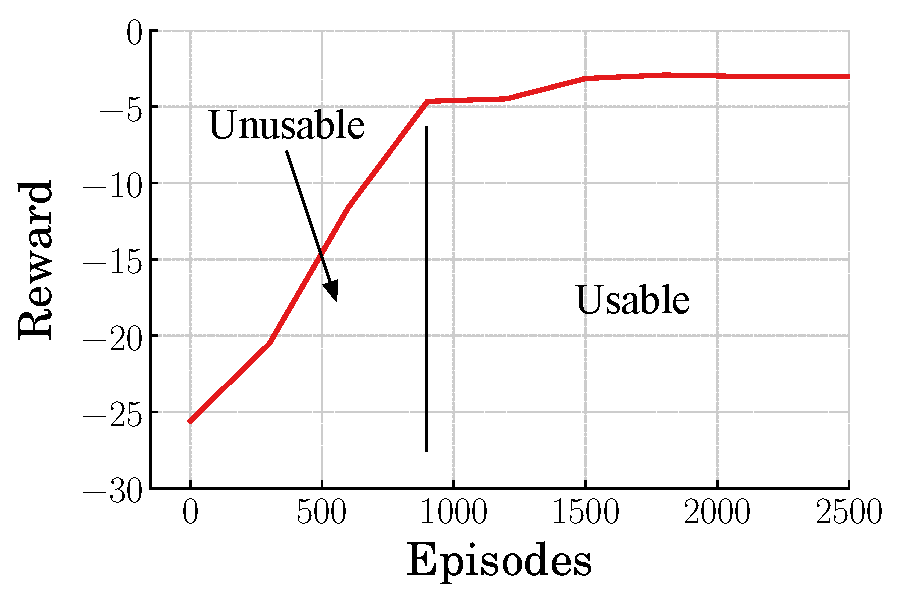
\includegraphics[width = 0.7\textwidth]{figures/figures_introduction/long_training_time}
\caption{Example of initial unusable policy} 
\label{fig_chap1:long_training_time}
\end{center}
\end{figure}
%

Another drawback to RL is the difficulty to develop performance guarantees for RL agents.
% \rph{It also tends to be difficult to develop performance guarantees for RL agents.}
In particular, the lack of stability guarantees prevents the adoption of RL in many applications.
Although some applications such as games do not require stability guarantees, physical applications, such as robotics and autonomous navigation, require stability guarantees in order to provide trust in the agent before implementation.
% \rnotes{In some cases we may want to guarantee stability over a certain operating region.} With standard RL algorithms, there is no way to guarantee how big the region of stability is. \rnotes{Post-hoc analysis after training runs into the standard difficulties for nonlinear systems.}
One method for training stable agents is to design a set of stabilizing controllers to serve as candidate controllers that the agent has to switch between~\cite{Perkins:2002a}. This method uses discrete actions to choose the appropriate stabilizing controller resulting in a discontinuous controller that is stable but suboptimal. Another method for learning stable agents involves providing an initial stabilizing policy and constraining any modification to the policy to remain stable~\cite{Berkenkamp:2017a}. As the agent learns, it is able to increase its approximated region of attraction. While this method provides safe and stabilizing agents within the region of attraction, it sacrifices exploration at the expense of stability. Additionally, a stabilizing initial policy must be provided. It is beneficial to have agents that achieve stability without having to pre-design stable policies for the RL controllers.

% \rnotes{Some work has tried to use different ways to parameterize RL to ensure stability~\cite{Friedrich:2017a}. I didn't completely understand those methods.}

RL agents also tend to be difficult to interpret, particularly deep RL agents. Because of the large number of nodes in a deep neural network required to model the policy, it is difficult to intuitively understand the control law learned by the agent, making the agent a black box~\cite{Alharin:2020a}. As with the inability to generate stability guarantees, this prevents the adoption of RL for many applications since it is difficult to predict the behavior of the agents in a wide range of scenarios. Some methods used to interpret agents require manual summarization of the behavior of the agent~\cite{Amir:2019a,Lage:2019a}. Other methods utilize decision trees, illustrated in Figure~\ref{fig_chap1:decision_tree}, which can help interpretability by reducing the complexity of the deep model into a concise graphical model~\cite{Bastani:2018a}.
%
Decision trees often require training a shallow model from a deep neural network model. However, agents with continuous action spaces or those that learn complex behaviors may require large decision trees that are still difficult to interpret.
%
% \what{Decision trees require training a shallow model from a deep neural network model. However, complex deep networks often require large decision trees, reducing the interpretability of the model~\pc.}

%
\begin{figure}[tb]
\begin{center}
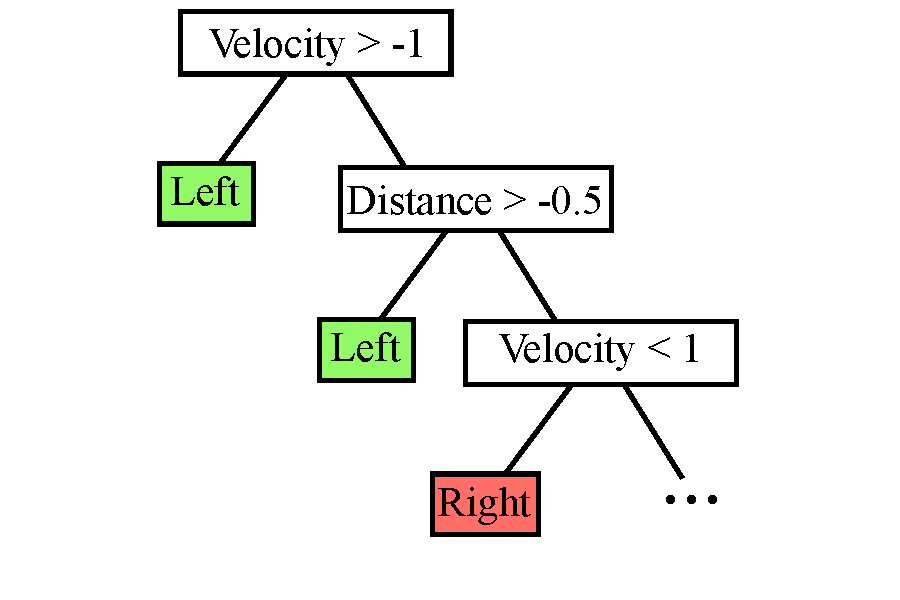
\includegraphics[width = 0.6\textwidth]{figures/figures_introduction/Decision_tree.pdf}
\caption{Example of a decision tree}
\label{fig_chap1:decision_tree}
\end{center}
\end{figure}
%

\section{Combining RL and Conventional Control}
\label{sec:combined_control_overview}

Although RL agents can learn policies without knowledge of the model of the system being controlled, a model is often available for use by the control systems designer. This is always the case for agents that are initially trained in simulation. Additionally, if a system model is known, an experienced controls engineer will also often have knowledge of how to design a controller that enables the system to accomplish the desired goal even if the controller is suboptimal.
%
RL controllers can be trained in a way to take advantage of established domain knowledge of dynamics and control theory. This can include direct design of controllers that combine RL and conventional control elements that both contribute to the total system input~\cite{Eaglin:2020a,Eaglin:2023a}. Domain knowledge may also be used indirectly through the design of the environment, such as reward function design. Domain knowledge can also be utilized in the analysis of agent performance after training to improve interpretability and generate performance guarantees. 

The following chapters present contributions that the combination of RL and conventional control have to the control design processes:
% Contributions of this work include:
\begin{itemize}
	\item Chapter~\ref{chapter2} introduces multiple controller architectures for combining RL with conventional control. The baseline performance of these combined controllers applied to multiple benchmark systems is then presented. The combined controllers are shown to generally reduce required training time to generate acceptable policies. Design guidelines are then presented based on the performance of the controllers.
	\item Chapter~\ref{chapter3} presents stability evaluations of the combined controllers.
	% Methods to design agents to satisfy certain stability conditions are also presented.
	\item Chapter~\ref{chapter4} presents the effects of the combined controllers on robustness to modeling error.
	\item Chapter~\ref{chapter5} proposes a method to use domain knowledge to improve interpretability of the learned controllers by approximating the agent with a piecewise set of control laws.
	\item Chapter~\ref{chapter6} presents an analysis of the current commercializability of this work.
\end{itemize}

% \begin{itemize}
% 	\item RL can be done model-free
% 	\item It does not require any knowledge of how to design control systems to train an agent
% 	\item But we often do have some idea how to design a control system for something
% 	\item We can use domain knowledge of dynamics and control to solve the problems listed above
% 	\item Combination of RL with domain knowledge can include
% 	\begin{itemize}
% 		\item Building a model/domain-knowledge-based controller directly to learn alongside the agent
% 		\item Informed design of other parts of the environment (like stability-based reward function)
% 		\item Post-hoc analysis and interpretation based on more properly understood methods
% 	\end{itemize}
% \end{itemize}

% \section{Contributions}

% {\color{red}The following chapters propose various methods used to plan trajectories for flexible mobile robots while limiting vibration. These include methods to limit vibration in trajectory tracking problems as well as planning paths which induce low vibration. While most work treats path planning and vibration control sequentially, these algorithms provide concurrent path planning and vibration control by incorporating explicit vibration constraints in the path planning algorithms.}

%
% \begin{table}[tb]
% \begin{center}
% \setlength{\tabcolsep}{15pt}
% \caption{Combined Controller ($K_{p}=5$) 5\% Settling Times}
% \vspace{-2ex}
% \begin{tabular}{l c c}
% \toprule
% \textbf{Step} & \textbf{5\% Settling Times (\si{\second})} & \textbf{Normalized}\\
% \midrule
% % $0$--$25$\si{\micro\meter} & \num{0.0017751}\\
% % $25$--$50$\si{\micro\meter} & \num{0.0017549}\\
% % $50$--$75$\si{\micro\meter} & \num{0.001446}\\
% % $75$--$100$\si{\micro\meter} & \num{0.0011047}\\
% $0$--$0.025$\si{\milli\meter} & \num{0.00178} & 0.88\\
% $0.025$--$0.5$\si{\milli\meter} & \num{0.00175} & 0.86\\
% $0.05$--$0.075$\si{\milli\meter} & \num{0.00145} & 1.99\\
% $0.075$--$0.1$\si{\milli\meter} & \num{0.00110} & 0.57\\
% \bottomrule
% \label{table:Combined_res_ch_Kp5}
% \end{tabular}
% \end{center}
% % \end{table}
% % %
% \vspace{-3ex}
% % \begin{table}[tb]
% \begin{center}
% \setlength{\tabcolsep}{15pt}
% \caption{Combined Controller ($K_{p}=10$) 5\% Settling Times}
% % \vspace{-1ex}
% \begin{tabular}{l c c}
% \toprule
% \textbf{Step} & \textbf{5\% Settling Times (\si{\second})} & \textbf{Normalized} \\
% \midrule
% % $0$--$25$\si{\micro\meter}  & \num{0.0011929}\\
% % $25$--$50$\si{\micro\meter}  & \num{0.0006639}\\
% % $50$--$75$\si{\micro\meter} & \num{0.0007425}\\
% % $75$--$100$\si{\micro\meter}  & \num{0.0007227}\\
% $0$--$0.025$\si{\milli\meter} & \num{0.00119} & 0.59\\
% $0.025$--$0.5$\si{\milli\meter} & \num{0.000664} & 0.33\\
% $0.05$--$0.075$\si{\milli\meter} & \num{0.000743} & 1.02\\
% $0.075$--$0.1$\si{\milli\meter} & \num{0.000723} & 0.37\\
% \bottomrule
% \label{table:Combined_res_ch_Kp10}
% \end{tabular}
% \end{center}
% \end{table}
% %


% \begin{figure}[tb]
% \begin{center}
% 	\begin{minipage}{0.45\textwidth}
% 	\begin{center}
% 	\includegraphics[width = \columnwidth]{figures/Chapter1_fig/Actuator_PID_with_shaping_Kp5_current}
% 	\caption{Current input for $K_{p}=5$}
% 	\label{fig:Actuator_PID_with_shaping_Kp5_current}
% 	\end{center}
% 	\end{minipage}
% \hspace{0.07\textwidth}
% 	\begin{minipage}{0.45\textwidth}
% 	\begin{center}
% 	\includegraphics[width = \columnwidth]{figures/Chapter1_fig/Actuator_PID_with_shaping_Kp10_current}
% 	\caption{Current input for $K_{p}=10$}
% 	\label{fig:Actuator_PID_with_shaping_Kp10_current}
% 	\end{center}
% 	\end{minipage}
% \end{center}
% \vspace{-0.2in}
% \end{figure}


% \begin{enumerate}
% 	\item \textbf{Development of an open-loop trajectory tracking method to minimize the tracking error of a flexible system} -- Chapter \ref{chapter2}
% 		\begin{itemize}	
% 			\item[] An open-loop vibration control method for trajectory tracking is presented. Trajectory tracking error resulting from vibration was minimized for arbitrary, pre-planned trajectories.
% 		\end{itemize}
% 	\item \textbf{Development of a discrete motion planner using vibration optimal movements} -- Chapter \ref{chapter3}
% 		\begin{itemize}
% 			\item [] An existing discrete path planner was adapted to plan paths that produce low-vibration. The new path planner generates trajectories such that vibration canceling pulses can be used to track the trajectory.
% 			% The planner utilizes movements which cancel vibration.
% 			This method is compared to input shaping to analyze time optimality.
% 		\end{itemize}
% 	\item \textbf{Development of an optimal sampling-based motion planner to produce continuous low-vibration trajectories} -- Chapter \ref{chapter4}
% 		\begin{itemize}
% 			\item[] A probabilistically complete sampling-based path planner which produces continuous trajectories for a flexible system is presented. Trajectories are planned while respecting kinematic and actuator constraints. A local planner is also presented to solve the two-point boundary value problem for flexible systems.
% 		\end{itemize}
% \end{enumerate}

% The next chapter will introduce a trajectory tracking method to minimize tracking error of systems following preplanned paths. Chapter \ref{chapter3} then introduces a discrete planning algorithm to generate paths that can be followed using a sequence of predefined optimal commands. This method generates trajectories that can be tracked with zero error. In Chapter \ref{chapter4}, a sampling-based algorithm modified from RRT and RRT* is discussed. This method generates low cost trajectories while accounting for actuator limits and velocity constraints. Chapter \ref{chapter5} then presents conclusions and potential future work.








% \begin{table}[t!]
% \centering
% \caption{Impulse Amplitudes and Spacing for Two Input Shaper}
% \label{table:multi-impulses}
% \begin{tabular}{@{}rrrr@{}}
% \toprule
% \multicolumn{1}{l}{} &  & \multicolumn{2}{c}{Impulse Amplitudes} \\ \midrule
% Impulse Times &  & Input $f_1$ & Input $f_2$ \\ \cmidrule(l){3-4} 
% 0 &  & 0.50 & 0.07 \\
% 0.84 &  & 0.09 & 0.94 \\
% 1.69 &  & 0.41 & 0.00 \\ \bottomrule
% \end{tabular}
% \end{table}